\textbackslash{}chapter\{The Calculus of Variations\}
\textbackslash{}label\{ch:2\}

2.2
Derivation of the Euler--Lagrange equation
As an analogy, let us recollect the introductory calculus method of finding
the maximum or minimum (that is, a ``stationary point'') of some function. For
example, consider an ordinary function, say h(x, y), which we will assume
represents a topological map with h being the altitude. Imagine a mountain
whose height is greater than the height of any other point on the map. That
is, at some point (say x0, y0) the height h is an absolute maximum. How can
we determine x0 and y0? As you know from elementary calculus, the technique is to find the point at which the partial derivatives of h with respect
to x and y are zero. (Clearly, as we go through a maximum, the slope of a
curve changes from positive to negative, so it must be zero at the maximum
itself.) But if the derivative of h with respect to x is zero, this means that
points that are infinitesimally distant from the peak along the x direction will
have the same value of h as the peak itself! That is, if \textbackslash{}partial h/\textbackslash{}partial x = 0, then there
is no change in h for a small change in x. To resolve this conundrum, we
note that near the peak, the function h(x, y) can be expanded in a Taylor's
series, thus,
h(x + dx, y + dy) = h(x0, y0) + dx \textbackslash{}partial h
\textbackslash{}partial x

x0,y0
+ dy \textbackslash{}partial h
\textbackslash{}partial y

x0,y0
+ second-order terms.
The derivatives \textbackslash{}partial h/\textbackslash{}partial x and \textbackslash{}partial h/\textbackslash{}partial x on the right-hand side are zero so in the
infinitesimal neighborhood of a stationary point the value of the function is, to
first order, equal to its value at the stationary point. To find a change in h we
need to go to the second-order terms. These terms will also tell us the nature
of the stationary point: if they are positive the stationary point is a minimum,
if they are negative it is a maximum and if they are positive in one direction
and negative in another, the stationary point is a saddle point.
Of course, we are not dealing with the problem of finding a stationary point
for a function, but rather for an integral. Furthermore, we are not varying the
coordinates, but rather the path along which the integral is evaluated. Nevertheless, to find the stationary point for our integral we will use the concept that
to first order the integral has the same value at all points in an infinitesimal
neighborhood of the stationary point.
\section*{2.2  Derivation of the Euler--Lagrange equation}

We now derive the basic equation of the calculus of variations. It is called
the Euler--Lagrange equation, or simply the Euler equation. As we derive the

relation, we shall try to make things more concrete by considering a simple
example, namely the problem of finding the length of the shortest curve
between two points in a plane. The curve is described by the function y =
y(x). An infinitesimal element of the curve has length ds, where
ds =

dx2 + dy2.
The length of the curve is, then,
I =
f
ds =
f

dx2 + dy2 =
f

1 +
dy
=
f

1 + y′2dx,
where the integral is taken between the end points (initial and final) of the
curve and the symbol y′ is defined to be y′ = dy
dx. (For convenience we denote
\begin{figure}[h]
\centering
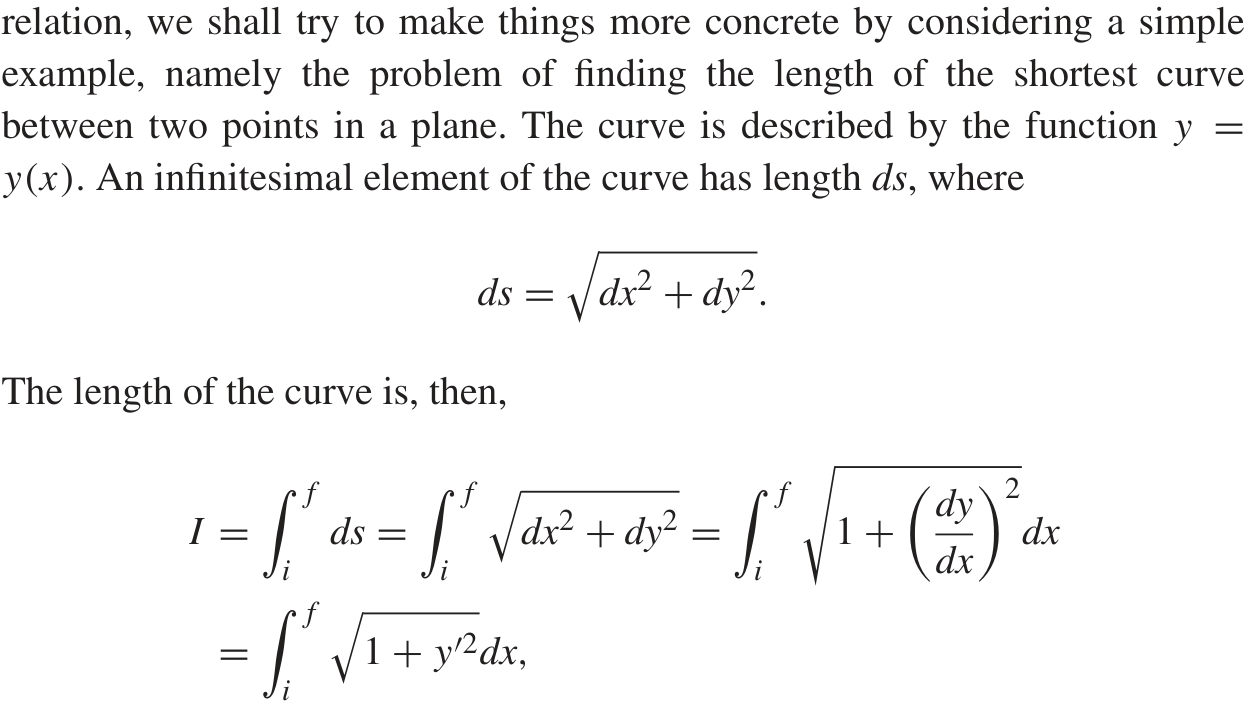
\includegraphics[width=0.55\linewidth]{../Figures/fig_2_1.png}
\caption{Figure 2.1}
\end{figure}

Now suppose you want to find the curve that corresponds to the shortest path
length between the two end points. That means you want to find a function
y = y(x) such that the integral I is a minimum.
The integral can be written in the following way
I =
f
(y) dx,
(2.1)
where  is a function of y. But y itself is a function (it is a function of x). So
is a function of a function. We call it a functional.
f
dy
ds
y
A curve y = y(x) between points i and f .

2.2
Derivation of the Euler--Lagrange equation
The problem is to find the function y(x) that minimizes the integral of
the functional (y). For the situation we are discussing, the functional is
obviously
(y) =

1 + y′2.
For different problems, as you can imagine, there are different functionals.
Here is a different problem. Determine the shape z = z(x) of a frictionless
wire such that a bead subjected to the gravitational force will slide from an
initial point ($\textbackslash{}xi$, zi) to a final point (xf , zf ) in the minimum amount of time.
(This is a famous problem that was solved by Isaac Newton in a few hours; it is
called the Brachistochrone problem.) In this problem we want to minimize the
time. The time it takes an object to go from one point to another is given by the
distance divided by the velocity. For a particle sliding down a wire the velocity
can be determined from conservation of energy in the form 1
2mv2 = mgh,
yielding
v =

2gh,
where h is the distance below the initial point. If we measure z downwards
from zi we can write v = \textbackslash{}sqrt2gz. The time to slide a distance ds along the
curve is, then,
dt =
ds
\textbackslash{}sqrt2gz =

dx2 + dz2
2gz
=

1 + z′2
2gz
dx.
The quantity to be minimized in this problem is
I =
f

1 + z′2
2gz
dx,
and the functional is
(z, z′) =

1 + z′2
2gz
.
(2.2)
\begin{example}
Example 2.1 A geodesic is the shortest distance between two points on a
spherical surface. This is a segment of a great circle. Eventually we will want
to determine the equation for a great circle, but here we will simply determine
the appropriate functional.

a
adq
a sin q
q
f
a sin q d f
ds
An element of path, ds, on the surface of a sphere.
Solution 2.1 An element of path on a sphere of radius a is denoted ds in
\begin{figure}[h]
\centering
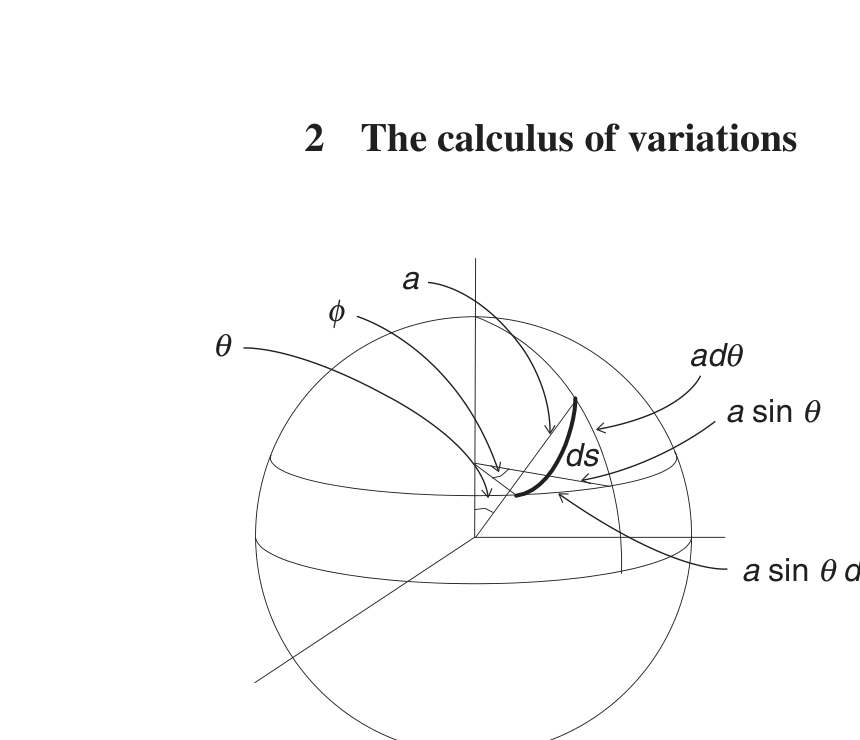
\includegraphics[width=0.55\linewidth]{../Figures/fig_2_2.png}
\caption{Figure 2.2}
\end{figure}

ds2 = a2d\textbackslash{}theta 2 + a2 sin2 \textbackslash{}theta d\textbackslash{}phi 2.
The length of a curve on the sphere is, therefore
I =

ds =

ad\textbackslash{}theta

1 + sin2 \textbackslash{}theta \textbackslash{}phi ′2,
where \textbackslash{}phi ′ = d\textbackslash{}phi /d\textbackslash{}theta . The functional is
=

1 + sin2 \textbackslash{}theta \textbackslash{}phi ′21/2
.
The functionals obtained in these examples are representative of those found
in calculus of variations problems. In general, the functionals we will be using
depend on two functions, such as y and y′, as well as the parameter x, thus:
= (x, y, y′).
(2.3)
Note that y = y(x) and y′ = y′(x) = dy(x)
dx . That is, x is the independent
parameter and y and y′ are functions of x. (Later we shall formulate problems
in which the independent parameter is the time, t.)
What we have done so far is to describe how the functional is obtained for
problems such as the shortest distance, the Brachistochrone and the geodesic.
We have not, however, shown how to determine the function that minimizes
the integral.

2.2
Derivation of the Euler--Lagrange equation
y
f
e = 0
A family of curves Y = y(x) + ϵ\textbackslash{}eta (x). The shortest distance curve
is indicated by ϵ = 0. Note that all the curves meet at the end points, so \textbackslash{}eta ($\textbackslash{}xi$) =
\textbackslash{}eta (xf ) = 0.
Let us now derive the condition for the integral to be stationary. I will use the
shortest path between two points as an example, but the derivation is general.
Imagine drawing a straight line between the points. As you know, this is the
path that gives the shortest distance. Imagine drawing nearby paths between the
same two points (i.e. paths that differ infinitesimally from the shortest path).
\begin{figure}[h]
\centering
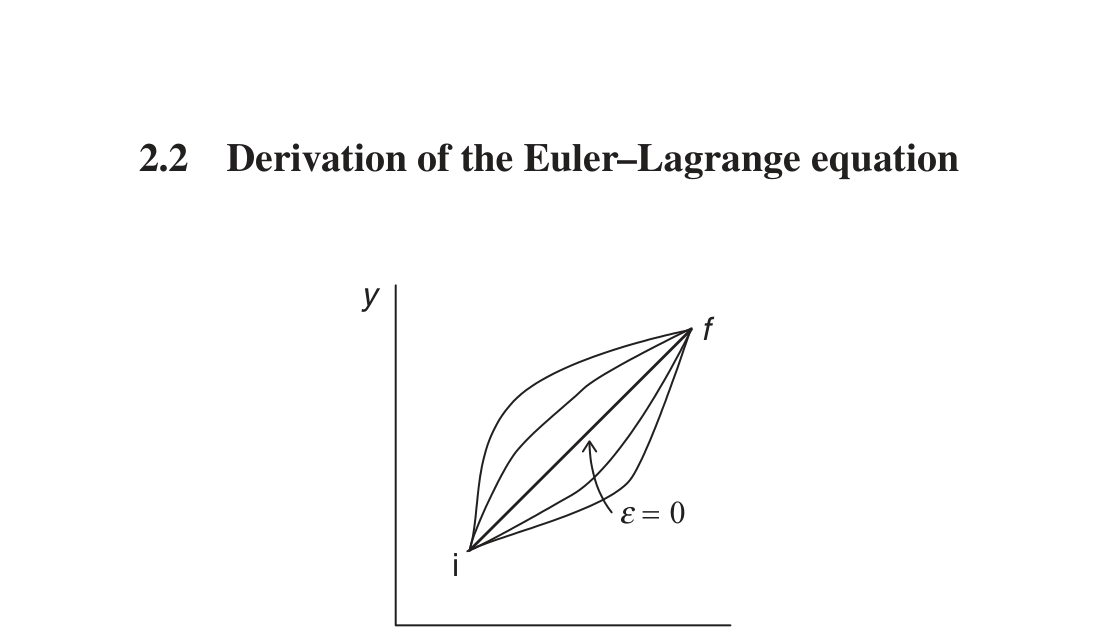
\includegraphics[width=0.55\linewidth]{../Figures/fig_2_3.png}
\caption{Figure 2.3}
\end{figure}

path. If y = y(x) is the equation of the minimal path, the equation of one of
the nearby paths can be expressed as
Y(x, ϵ) = y(x) + ϵ\textbackslash{}eta (x),
(2.4)
where ϵ is a small quantity and \textbackslash{}eta (x) is an arbitrary function of x but which
has an important condition on it, namely that \textbackslash{}eta (x) must be zero at the end
points because at those points the paths all meet. For a given function \textbackslash{}eta (x),
different values of ϵ will yield different paths, all belonging to same family
of curves. (Selecting a different function \textbackslash{}eta (x) will generate another family of
curves, each characterized by the value of ϵ.) Assuming a given \textbackslash{}eta (x), the path
Y(x) is a function of ϵ as well as x. That is why we wrote Y = Y(x, ϵ). The
length of any one of these curves will, of course, depend on the value of ϵ and
can be expressed as
I(ϵ) =
xf
(x, Y, Y ′)dx,
where  has the form
=

1 + Y ′2.
We wrote I as a function only of ϵ because the dependence on x has been
integrated out.

We want to determine the function y(x) that makes the integral I stationary.
In ordinary calculus we would set the differential to zero (dI = 0). But now
we are asking which of the functions y(x) makes I stationary, so we set the
variation to zero (\textbackslash{}delta I = 0). This is often called the ``first variation'' because \textbackslash{}delta I
is defined in terms of the Maclaurin expansion
I(ϵ) = I(0) +

dϵ

ϵ=0
ϵ + O(ϵ2).
Keeping only the first term in ϵ we define
\textbackslash{}delta I(ϵ) = I(ϵ) -I(0) =

dϵ

ϵ=0
ϵ.
Consequently, \textbackslash{}delta I = 0 is equivalent to
dI
dϵ

ϵ=0 = 0.
Inserting the integral expression for I, gives us

dϵ
xf
(x, Y, Y ′)dx

ϵ=0
= 0.
(2.5)
Y and Y ′ are both functions of ϵ. Taking the derivative under the integral
we have
xf

\textbackslash{}partial
\textbackslash{}partial Y
\textbackslash{}partial Y
\textbackslash{}partial ϵ + \textbackslash{}partial
\textbackslash{}partial Y ′
\textbackslash{}partial Y ′
\textbackslash{}partial ϵ

ϵ=0
dx = 0.
(2.6)
The second term can be integrated by parts as follows:
xf

\textbackslash{}partial
\textbackslash{}partial Y ′
\textbackslash{}partial Y ′
\textbackslash{}partial ϵ

dx =
xf
\textbackslash{}partial
\textbackslash{}partial Y ′
\textbackslash{}partial
\textbackslash{}partial ϵ
dY

dx =
xf
\textbackslash{}partial
\textbackslash{}partial Y ′
\textbackslash{}partial Y
\textbackslash{}partial ϵ

=
xf
\textbackslash{}partial
\textbackslash{}partial Y ′ d
\textbackslash{}partial Y
\textbackslash{}partial ϵ

= \textbackslash{}partial
\textbackslash{}partial Y ′
\textbackslash{}partial Y
\textbackslash{}partial ϵ

xf
-
xf
\textbackslash{}partial
\textbackslash{}partial Y ′
\textbackslash{}partial Y
\textbackslash{}partial ϵ dx.
But Y = y(x) + ϵ\textbackslash{}eta (x) so \textbackslash{}partial Y
\textbackslash{}partial ϵ = \textbackslash{}eta (x) and at the end points \textbackslash{}eta (x) = 0 (because
the curves meet there). Hence
\textbackslash{}partial
\textbackslash{}partial Y ′
\textbackslash{}partial Y
\textbackslash{}partial ϵ

xf
= \textbackslash{}partial
\textbackslash{}partial Y ′

\textbackslash{}eta (xf ) -\textbackslash{}eta ($\textbackslash{}xi$)

= 0.
Consequently, Equation (2.6) is
xf

\textbackslash{}partial
\textbackslash{}partial Y -d

\textbackslash{}partial
\textbackslash{}partial Y ′
\textbackslash{}partial Y
\textbackslash{}partial ϵ

ϵ=0
dx = 0.
(2.7)

2.2
Derivation of the Euler--Lagrange equation
The integrand is the product of two functions. Since \textbackslash{}partial Y
\textbackslash{}partial ϵ = \textbackslash{}eta (x), Equation (2.7)
has the form
b
a
f (x)\textbackslash{}eta (x)dx = 0,
(2.8)
where
f (x) = \textbackslash{}partial
\textbackslash{}partial Y -d
\textbackslash{}partial
\textbackslash{}partial Y ′

.
The function \textbackslash{}eta (x) is arbitrary (except at the end points) so Equation (2.8) can
be true if and only if f (x) = 0 for all values of x. You might think that requiring f (x) = 0 for all x is too restrictive, but it is easy to show that it is not. You
can appreciate this by assuming \textbackslash{}eta (x) is zero everywhere except at some point
between $\textbackslash{}xi$ and xf , say at x = \textbackslash{}xi . Next consider the integral
xf =\textbackslash{}xi +\textbackslash{}epsilon
$\textbackslash{}xi$=\textbackslash{}xi -\textbackslash{}epsilon
f (x)\textbackslash{}eta (x)dx = 0,
where \textbackslash{}epsilon  is a very small quantity. Since the integral is zero everywhere, it is
zero in the range of integration. Furthermore, f (x) is essentially constant over
the small region of integration. Denote it by f (\textbackslash{}xi ) and take it outside the integral sign,
f (\textbackslash{}xi )
xf =\textbackslash{}xi +\textbackslash{}epsilon
$\textbackslash{}xi$=\textbackslash{}xi -\textbackslash{}epsilon
\textbackslash{}eta (x)dx = 0.
The integral is not zero, so f (\textbackslash{}xi ) must be zero. But the point x = \textbackslash{}xi  could be
anywhere in the interval $\textbackslash{}xi$ to xf , so f (x) is zero at all points along the path.
Another argument that
b
a f (x)\textbackslash{}eta (x)dx = 0 implies f (x) = 0 is to assume
that f (x) is not zero and use the fact that \textbackslash{}eta (x) is arbitrary. For example, we
could require that \textbackslash{}eta (x) be negative everywhere that f (x) is negative and that
\textbackslash{}eta (x) be positive wherever f (x) is positive. But then the product f (x)\textbackslash{}eta (x)
would be positive everywhere and the condition (2.8) would not be met. Once
again, we conclude that Equation (2.8) is true if and only if f (x) = 0. Consequently, Equation (2.7) reduces to

\textbackslash{}partial
\textbackslash{}partial Y -d
\textbackslash{}partial
\textbackslash{}partial Y ′

ϵ=0
= 0,
which is equivalent to requiring that
\textbackslash{}partial
\textbackslash{}partial y -d
\textbackslash{}partial
\textbackslash{}partial y′

= 0.
(2.9)

This is called the Euler--Lagrange equation.1 It gives a condition that must be
met if y = y(x) is the path that minimizes the integral
xf
(x, y, y′)dx.
For example, in determining the equation for the minimal distance between
two points in a plane, the functional was
(x, y, y′) =

1 + y′2.
Plugging this into the Euler--Lagrange equation we obtain
-d
\textbackslash{}partial
\textbackslash{}partial y′

1 + y′2 1
2 = 0,
and this leads, after a bit of algebra, to
y = mx + b,
where m and b are constants. But y = mx +b is the equation of a straight line!
\end{example}

\begin{exercise}
Exercise 2.1 Show that the functional  =

1 + y′2 leads to y = mx+b.
\end{exercise}

\begin{exercise}
Exercise 2.2 Find the equation for the shortest distance between two
points in a plane using polar coordinates. Answer: r cos(\textbackslash{}theta  + \textbackslash{}alpha ) = C,
where \textbackslash{}alpha  and C are constants.
\end{exercise}

\begin{exercise}
Exercise 2.3 Determine and identify the curve y
= y(x) such that
x2
x1 [x(1 + y′2)]1/2dx is stationary. Answer: A parabola.
\end{exercise}

\begin{exercise}
Exercise 2.4 Determine and identify the curve y = y(x) such that
x2
x1
ds
is stationary. Answer: A circle.
2.2.1 The difference between \textbackslash{}delta  and d
The difference between \textbackslash{}delta  and d is more than notational.
When applied to a variable, \textbackslash{}delta  represents a virtual displacement, which we
usually think of as a change in a coordinate carried out with time frozen. More
generally, it is an infinitesimal change in some variable that is virtual; that
1 You have met a variant of the Euler--Lagrange equation in Chapter 1 (Equation (1.16)).

2.2
Derivation of the Euler--Lagrange equation
is, carried out in an arbitrary but kinematically allowable manner while keeping the independent parameter constant. In contrast, we think of d as representing an actual change in a variable which occurs during some finite period
of time.
When applied to a function, the symbol \textbackslash{}delta , which was introduced by
Lagrange, represents the variation of the function, whereas d is the differential
of the function. As a simple example, consider the function F(x, $\textbackslash{}dot x$, t), that is
a function that depends on position, velocity and time. But position and velocity both depend on time. That is, time is the independent parameter, and we
can write
F = F(x(t), $\textbackslash{}dot x$(t), t).
According to the rules of calculus, the differential of F is
dF = \textbackslash{}partial F
\textbackslash{}partial x dx + \textbackslash{}partial F
\textbackslash{}partial $\textbackslash{}dot x$ d $\textbackslash{}dot x$ + \textbackslash{}partial F
\textbackslash{}partial t dt.
On the other hand, the variation of F is
\textbackslash{}delta F = \textbackslash{}partial F
\textbackslash{}partial x \textbackslash{}delta x + \textbackslash{}partial F
\textbackslash{}partial $\textbackslash{}dot x$ \textbackslash{}delta  $\textbackslash{}dot x$.
The most significant difference between the differential and the variation is
that the differential takes us to a different point of the same function whereas
\begin{figure}[h]
\centering
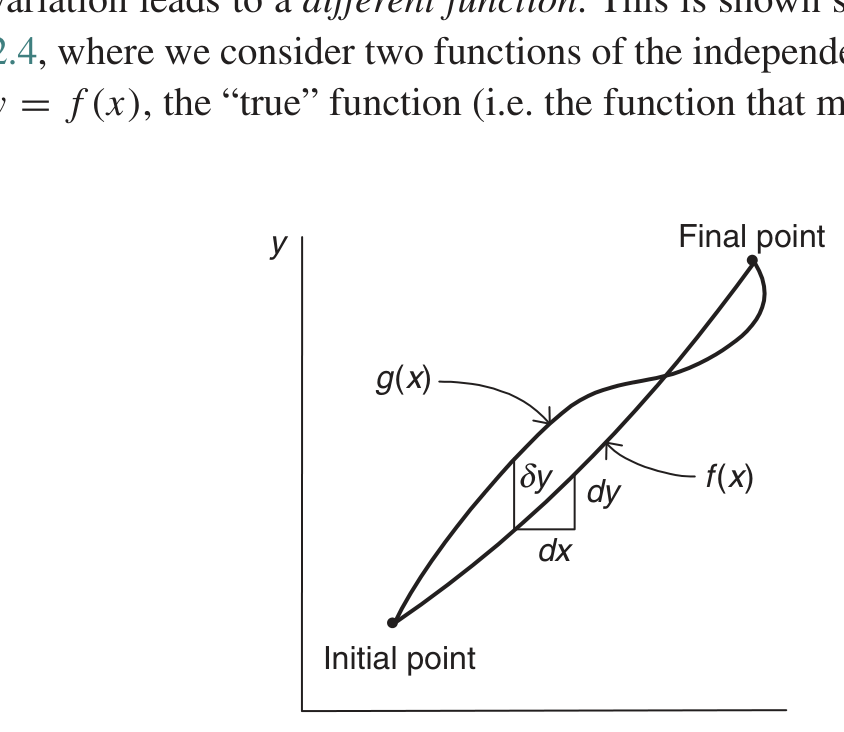
\includegraphics[width=0.55\linewidth]{../Figures/fig_2_4.png}
\caption{Figure 2.4}
\end{figure}

are y = f (x), the ``true'' function (i.e. the function that minimizes the definite
dy
f(x)
g(x)
Initial point
Final point
y
dy
An illustration of the difference between \textbackslash{}delta  and d.

integral) and y = g(x) = f (x) + ϵ\textbackslash{}eta (x), which is a nearby function with the
same end points, i.e. the ``varied'' function. The variation \textbackslash{}delta y is given by
\textbackslash{}delta y = g(x) -f (x).
That is, \textbackslash{}delta y gives the difference between the true function and the varied function at the same value of x. On the other hand, if y = f (x), then dy is the
change in f (x) due to a change in x. That is
dy = f (x + dx) -f (x).
The difference between \textbackslash{}delta  and d becomes particularly important when
applied to definite integrals because both kinds of changes are often acting
simultaneously.
In the derivation of the Euler--Lagrange equation we used ϵ as a parameter
that indicated whether or not we were on the ``true'' path (for which ϵ = 0)
or on one of the varied paths (ϵ̸ = 0). It is clear that the integral I giving
the length of a path depends on ϵ. That is why we wrote I = I(ϵ). Our next
step was to take the derivative of I with respect to ϵ and set it equal to zero.
(The different values of ϵ take us to different curves, i.e. to different functions
y = y(x).)
We could also have expressed our problem in terms of variations, such as
\textbackslash{}delta y = \textbackslash{}eta (x)dϵ,
and
\textbackslash{}delta y′ = \textbackslash{}eta ′(x)dϵ.
These relations agree with the expression Y(x) = y(x) + ϵ\textbackslash{}eta (x). If we recall
that Y(x) represents a family of curves y(x, ϵ), then replacing Y(x) with
y(x, ϵ) we have
\textbackslash{}delta y = \textbackslash{}delta [y(x, ϵ)] =

dy(x, ϵ)
dϵ

ϵ=0
\textbackslash{}delta ϵ =

dϵ (y(x) + ϵ\textbackslash{}eta (x))

ϵ=0
\textbackslash{}delta ϵ = \textbackslash{}eta (x)\textbackslash{}delta ϵ.
Since I = I(y, y′, x) we have
\textbackslash{}delta I = \textbackslash{}partial I
\textbackslash{}partial y \textbackslash{}delta y + \textbackslash{}partial I
\textbackslash{}partial y′ \textbackslash{}delta y′.
(Note that x is frozen.) But
\textbackslash{}delta I = \textbackslash{}delta
x2
x1
(y, y′, x)dx
=
x2
x1
\textbackslash{}delta dx

2.2
Derivation of the Euler--Lagrange equation
=
x2
x1
\textbackslash{}partial
\textbackslash{}partial y \textbackslash{}delta y + \textbackslash{}partial
\textbackslash{}partial y′ \textbackslash{}delta y′

=
x2
x1

\textbackslash{}partial
\textbackslash{}partial y \textbackslash{}eta (x)dϵ + \textbackslash{}partial
\textbackslash{}partial y′ \textbackslash{}eta ′(x)dϵ

dx.
Thus we could express the condition on I in either one of two ways, namely
by setting

dϵ

ϵ=0
= 0
as we did in Equation (2.7), or by stating that the variation \textbackslash{}delta I is zero. These
two statements are equivalent.
A final comment on notation. The ``functional derivative'' of  = (y, y′, x)
is defined by
\textbackslash{}delta
\textbackslash{}delta y = \textbackslash{}partial
\textbackslash{}partial y -d
\textbackslash{}partial
\textbackslash{}partial y′ .
(2.10)
This is sometimes called the ``variational derivative.''
\end{exercise}

\begin{exercise}
Exercise 2.5 Show that \textbackslash{}delta  and d commute.
\end{exercise}

\begin{exercise}
Exercise 2.6 Given
\textbackslash{}delta  = \textbackslash{}partial
\textbackslash{}partial y \textbackslash{}delta y + \textbackslash{}partial
\textbackslash{}partial y′ \textbackslash{}delta y′,
demonstrate that \textbackslash{}delta I = 0 means the same thing as
dI
dϵ

ϵ=0 = 0.
2.2.2 Alternate forms of the Euler--Lagrange equation
We derived the Euler--Lagrange equation in the form
\textbackslash{}partial
\textbackslash{}partial y -d
\textbackslash{}partial
\textbackslash{}partial y′

= 0.
There are two variants of this expression. One of them is useful for problems
in which  does not depend on y and the other is useful for problems in which
does not depend on x.
If  does not depend on y, the Euler--Lagrange equation reduces to
\textbackslash{}partial
\textbackslash{}partial y′

= 0,

from which we conclude that
\textbackslash{}partial
\textbackslash{}partial y′ = constant.
(This was the situation when we solved the ``shortest distance in a plane''
problem.)
Next assume that  does not depend on x. Then, since  = (y, y′), the
partial derivative of  with respect to x is zero and the total derivative of
with respect to x will be
d
dx = \textbackslash{}partial
\textbackslash{}partial y
dy
dx + \textbackslash{}partial
\textbackslash{}partial y′
dy′
dx .
But dy′
dx = d
dy
dx = y′′, so
d
dx = \textbackslash{}partial
\textbackslash{}partial y
dy
dx + y′′ \textbackslash{}partial
\textbackslash{}partial y′ = y′ \textbackslash{}partial
\textbackslash{}partial y + y′′ \textbackslash{}partial
\textbackslash{}partial y′ .
(2.11)
If we multiply the Euler--Lagrange equation by y′ we obtain
y′ \textbackslash{}partial
\textbackslash{}partial y -y′ d
\textbackslash{}partial
\textbackslash{}partial y′

= 0.
Add y′′ \textbackslash{}partial
\textbackslash{}partial y′ to both sides:
y′ \textbackslash{}partial
\textbackslash{}partial y -y′ d
\textbackslash{}partial
\textbackslash{}partial y′

+ y′′ \textbackslash{}partial
\textbackslash{}partial y′ = y′′ \textbackslash{}partial
\textbackslash{}partial y′
y′ \textbackslash{}partial
\textbackslash{}partial y + y′′ \textbackslash{}partial
\textbackslash{}partial y′ = y′′ \textbackslash{}partial
\textbackslash{}partial y′ + y′ d
\textbackslash{}partial
\textbackslash{}partial y′

.
The left-hand side is just d
dx (see Equation (2.11)) and the right-hand side is

y′ \textbackslash{}partial
\textbackslash{}partial y′

, so
d
dx = d

y′ \textbackslash{}partial
\textbackslash{}partial y′

,
or

-y′ \textbackslash{}partial
\textbackslash{}partial y′

= 0.
Therefore,
-y′ \textbackslash{}partial
\textbackslash{}partial y′ = constant.
(2.12)

2.2
Derivation of the Euler--Lagrange equation
\end{exercise}

\begin{example}
Example 2.2 The Brachistochrone problem: The problem is to determine the
shape of a wire such that a bead on the wire will slide from some initial point to
some lower final point in the least amount of time. Note that the two end points
(x1, z1) and (x2, z2) are fixed. In Section 2.2 we obtained the functional. We
now solve for the curve z = z(x).
Solution 2.2 The functional was given by Equation (2.2) as
(z, z′) =

1 + z′2
2gz .
Note that  does not depend on x. Therefore,
-z′ \textbackslash{}partial
\textbackslash{}partial z′ = constant.
The factor 2g can be discarded. Carrying out the mathematics, we obtain

1 + z′2
z
-
z′2
\textbackslash{}sqrtz\textbackslash{}sqrt
1 + z′2 = constant = 1/C.
(2.13)
This can be expressed as
z(1 + z′2) = C.
(2.14)
The details are left as an exercise. We can obtain a solution to this differential
equation by setting
z′ = cot \textbackslash{}theta .
Then 1 + z′2 = 1/ sin2 \textbackslash{}theta , and our differential equation can be written
z(1 + cot2 \textbackslash{}theta ) = z/ sin2 \textbackslash{}theta  = C,
or
z = C sin2 \textbackslash{}theta .
Next note that
d\textbackslash{}theta  = dx
dz
dz
d\textbackslash{}theta  = 1
z′
dz
d\textbackslash{}theta  = tan \textbackslash{}theta  dz
d\textbackslash{}theta  = tan \textbackslash{}theta  d
d\textbackslash{}theta  (C2 sin2 \textbackslash{}theta ) = C(1 -cos 2\textbackslash{}theta ).
Therefore
x =

C(1 -cos 2\textbackslash{}theta )d\textbackslash{}theta  = C

\textbackslash{}theta  -sin 2\textbackslash{}theta

.

Letting C = 2A and 2\textbackslash{}theta  = \textbackslash{}phi  we can write the following parametric equations
for x and z:
x = A(\textbackslash{}phi  -sin \textbackslash{}phi )
z = A(1 -cos \textbackslash{}phi ).
These are the parametric equations for a cycloid. Consequently, the bead slides
in minimum time from (x1, z1) to (x2, z2) if the wire is bent into a cycloid.
\end{example}

\begin{exercise}
Exercise 2.7 Show the equivalence of the following two forms of the
Euler--Lagrange equation
\textbackslash{}partial
\textbackslash{}partial y -d
\textbackslash{}partial
\textbackslash{}partial y′ = 0
and
\textbackslash{}partial
\textbackslash{}partial x -d

-y′ \textbackslash{}partial
\textbackslash{}partial y′

= 0,
assuming y′̸ = 0.
\end{exercise}

\begin{exercise}
Exercise 2.8 Obtain Equation (2.14) starting with Equation (2.13).
\end{exercise}

\begin{exercise}
Exercise 2.9 Determine the minimum time for a bead to slide down a wire
from the point (-\textbackslash{}pi , 2) to (0, 0) (meters). Answer: \textbackslash{}pi /\textbackslash{}sqrtg.
\end{exercise}

\section*{2.3  Generalization to several dependent variables}

We have been considering problems whose functionals have the form  =
(x, y, y′). In this section we generalize to functionals that depend on n
dependent variables, y1, y2, . . . , yn and their derivatives, y′
1, y′
2, . . . , y′
n. We
assume the variables are independent.2
The functional for the system is now (y1, y2, . . . , yn, y′
1, y′
2, . . . , y′
n, x).
We will show that this leads to n Euler--Lagrange equations of the form:
\textbackslash{}partial
\textbackslash{}partial y′

-\textbackslash{}partial
\textbackslash{}partial yi
= 0,
i = 1, . . . , n.
2 This section is included for the sake of completeness. The procedure is a generalization of the
the simpler situation described in the the previous section (2.2). You may skip this section
without loss of continuity, but note that some of the results obtained here are used in
Section 3.4.

2.3
Generalization to several dependent variables
The derivation is similar to that presented in the preceding section, but is more
general.
Recall that our intention is to determine the functions y1(x), y2(x), . . . which
will minimize (or maximize) the definite integral
I =
xf
(y1, . . . , yn, y′
1, . . . , y′
n, x)dx.
That is, we want to obtain the functions yi(x) such that
\textbackslash{}delta I = 0.
As before, there are an infinite number of paths between the end points.
The paths that are infinitesimally near the minimal or true path can be
described by
Yi(x) = yi(x) + ϵ\textbackslash{}eta i(x).
The integral I depends on which path is chosen, so it can be considered a
function of ϵ.
The variation of I is
\textbackslash{}delta I = \textbackslash{}delta
xf
dx =
xf
\textbackslash{}delta dx =
xf

\textbackslash{}partial
\textbackslash{}partial Yi
\textbackslash{}delta Yi + \textbackslash{}partial
\textbackslash{}partial Y ′
\textbackslash{}delta Y ′

dx.
Considering Yi and Y ′
i as functions of ϵ, we write
\textbackslash{}delta I =
\textbackslash{}partial I
\textbackslash{}partial ϵ

ϵ=0
dϵ =
xf

\textbackslash{}partial
\textbackslash{}partial Yi
\textbackslash{}partial Yi
\textbackslash{}partial ϵ + \textbackslash{}partial
\textbackslash{}partial Y ′
\textbackslash{}partial Y ′
\textbackslash{}partial ϵ


ϵ=0
dϵ.
The second term can be integrated by parts. (Note that the mathematical procedure here is nearly identical to that from Equation (2.6) to Equation (2.7).)
We have
xf
\textbackslash{}partial
\textbackslash{}partial Y ′
\textbackslash{}partial Y ′
\textbackslash{}partial ϵ dϵdx =
xf
\textbackslash{}partial
\textbackslash{}partial Y ′
\textbackslash{}partial 2Yi
\textbackslash{}partial ϵ\textbackslash{}partial x dxdϵ =
xf
\textbackslash{}partial
\textbackslash{}partial Y ′
\textbackslash{}partial
\textbackslash{}partial ϵ
\textbackslash{}partial Yi
\textbackslash{}partial x dx

dϵ
= \textbackslash{}partial
\textbackslash{}partial Y ′
\textbackslash{}partial Yi
\textbackslash{}partial ϵ

x2
x1
-
xf
\textbackslash{}partial Yi
\textbackslash{}partial ϵ
\textbackslash{}partial
\textbackslash{}partial Y ′
dxdϵ
= -
xf
\textbackslash{}partial Yi
\textbackslash{}partial ϵ
\textbackslash{}partial
\textbackslash{}partial Y ′
dxdϵ,
where we have used the fact that \textbackslash{}partial Yi
\textbackslash{}partial ϵ

x2
x1
= 0 because all the curves pass through
the end points.

Consequently,
\textbackslash{}delta I =
xf

\textbackslash{}partial
\textbackslash{}partial Yi
\textbackslash{}partial Yi
\textbackslash{}partial ϵ -\textbackslash{}partial Yi
\textbackslash{}partial ϵ
\textbackslash{}partial
\textbackslash{}partial Y ′

dϵdx
=
xf

\textbackslash{}partial
\textbackslash{}partial Yi
-d
\textbackslash{}partial
\textbackslash{}partial Y ′
\textbackslash{}partial Yi
\textbackslash{}partial ϵ dϵdx
=
xf

\textbackslash{}partial
\textbackslash{}partial Yi
-d
\textbackslash{}partial
\textbackslash{}partial Y ′

\textbackslash{}delta Yidx.
When ϵ = 0, \textbackslash{}delta I = 0 because I is minimized along the path yi = yi(x). So
[\textbackslash{}delta I]ϵ=0 = 0 =
xf

\textbackslash{}partial
\textbackslash{}partial yi
-d
\textbackslash{}partial
\textbackslash{}partial y′

\textbackslash{}delta yidx.
(2.15)
Since the \textbackslash{}delta yis are independent, the only way this expression can be zero is for
all the terms in the parenthesis to be zero. Hence,
\textbackslash{}partial
\textbackslash{}partial yi
-d
\textbackslash{}partial
\textbackslash{}partial y′

= 0,
i = 1, . . . , n,
(2.16)
as expected.
\section*{2.4  Constraints}

Many problems in the calculus of variations involve constraints or, as they
are sometimes called, ``auxiliary conditions.'' For example, a particle might be
constrained to the z = 0 plane or to move along a specific curve.
2.4.1 Holonomic constraints
Let us begin by considering holonomic constraints. Recall from Section 1.4
that a holonomic constraint is a relationship between the dependent variables
that can be expressed as a function that is equal to zero. In the presence of a
constraint, the dependent variables are not independent of one another, being
related by the auxiliary conditions. For example, let us consider a problem
described by  = (y1, . . . , yn; y′
1, . . . , y′
n; x) where the n dependent variables are related by m constraints of the form
f1(y1, y2, . . . , yn, x) = 0,
...
fm(y1, y2, . . . , yn, x) = 0.

2.4
Constraints
Each constraint reduces by one the number of degrees of freedom. If there
are n dependent coordinates and m constraints we can use the constraints to
reduce the number of degrees of freedom to n -m and then apply n -m
Euler--Lagrange equations to solve the problem. This is conceptually simple,
but may be fairly complicated in practice. A better approach is to keep all n
variables and use the method of Lagrange multipliers. We now consider this
method (often referred to as Lagrange's \textbackslash{}lambda -method). We begin by taking the
variation of the constraint equations, thus:
\textbackslash{}delta f1 = \textbackslash{}partial f1
\textbackslash{}partial y1
\textbackslash{}delta y1 + \textbackslash{}partial f1
\textbackslash{}partial y2
\textbackslash{}delta y2 + \textbackslash{}cdot  \textbackslash{}cdot  \textbackslash{}cdot  + \textbackslash{}partial f1
\textbackslash{}partial yn
\textbackslash{}delta yn = 0,
...
\textbackslash{}delta fm = \textbackslash{}partial fm
\textbackslash{}partial y1
\textbackslash{}delta y1 + \textbackslash{}partial fm
\textbackslash{}partial y2
\textbackslash{}delta y2 + \textbackslash{}cdot  \textbackslash{}cdot  \textbackslash{}cdot  + \textbackslash{}partial fm
\textbackslash{}partial yn
\textbackslash{}delta yn = 0.
(2.17)
Next, we multiply each of these relations by an ``undetermined multiplier'' \textbackslash{}lambda i
and sum them to obtain
\textbackslash{}lambda 1\textbackslash{}delta f1 + \textbackslash{}lambda 2\textbackslash{}delta f2 + \textbackslash{}cdot  \textbackslash{}cdot  \textbackslash{}cdot  + \textbackslash{}lambda m\textbackslash{}delta fm = 0.
(2.18)
The sum is zero because each \textbackslash{}delta f is zero.
We also know that the variation of the functional  vanishes at the stationary
point. That is,
\textbackslash{}delta  = \textbackslash{}partial
\textbackslash{}partial y1
\textbackslash{}delta y1 + \textbackslash{}partial
\textbackslash{}partial y2
\textbackslash{}delta y2 + \textbackslash{}cdot  \textbackslash{}cdot  \textbackslash{}cdot  + \textbackslash{}partial
\textbackslash{}partial yn
\textbackslash{}delta yn = 0.
(2.19)
The sum of Equations (2.18) and (2.19) must also be zero, so we have
0 = \textbackslash{}partial
\textbackslash{}partial y1
\textbackslash{}delta y1 + \textbackslash{}partial
\textbackslash{}partial y2
\textbackslash{}delta y2 + \textbackslash{}cdot  \textbackslash{}cdot  \textbackslash{}cdot  + \textbackslash{}partial
\textbackslash{}partial yn
\textbackslash{}delta yn
+ \textbackslash{}lambda 1
\textbackslash{}partial f1
\textbackslash{}partial y1
\textbackslash{}delta y1 + \textbackslash{}partial f1
\textbackslash{}partial y2
\textbackslash{}delta y2 + \textbackslash{}cdot  \textbackslash{}cdot  \textbackslash{}cdot  + \textbackslash{}partial f1
\textbackslash{}partial yn
\textbackslash{}delta yn

+ \textbackslash{}cdot  \textbackslash{}cdot  \textbackslash{}cdot  + \textbackslash{}lambda m
\textbackslash{}partial fm
\textbackslash{}partial y1
\textbackslash{}delta y1 + \textbackslash{}partial fm
\textbackslash{}partial y2
\textbackslash{}delta y2 + \textbackslash{}cdot  \textbackslash{}cdot  \textbackslash{}cdot  + \textbackslash{}partial fm
\textbackslash{}partial yn
\textbackslash{}delta yn

.
(2.20)
The expression is complicated so, to illustrate the procedure, I will assume
that there is a single constraint. (The generalization to m constraints is left as
a problem.) If there is only one constraint, Equation (2.18) can be written as
\textbackslash{}lambda \textbackslash{}delta f = \textbackslash{}lambda
\textbackslash{}partial f
\textbackslash{}partial y1
\textbackslash{}delta y1 + \textbackslash{}partial f
\textbackslash{}partial y2
\textbackslash{}delta y2 + \textbackslash{}cdot  \textbackslash{}cdot  \textbackslash{}cdot  + \textbackslash{}partial f
\textbackslash{}partial yn
\textbackslash{}delta yn

= 0,
(2.21)

and Equation (2.20) reduces to
\textbackslash{}partial
\textbackslash{}partial y1
\textbackslash{}delta y1 + \textbackslash{}partial
\textbackslash{}partial y2
\textbackslash{}delta y2 + \textbackslash{}cdot  \textbackslash{}cdot  \textbackslash{}cdot  + \textbackslash{}partial
\textbackslash{}partial yn
\textbackslash{}delta yn
+ \textbackslash{}lambda
\textbackslash{}partial f
\textbackslash{}partial y1
\textbackslash{}delta y1 + \textbackslash{}partial f
\textbackslash{}partial y2
\textbackslash{}delta y2 + \textbackslash{}cdot  \textbackslash{}cdot  \textbackslash{}cdot  + \textbackslash{}partial f
\textbackslash{}partial yn
\textbackslash{}delta yn

= 0.
Re-arranging yields
n

i=1
\textbackslash{}partial
\textbackslash{}partial yi
+ \textbackslash{}lambda  \textbackslash{}partial f
\textbackslash{}partial yi

\textbackslash{}delta yi = 0.
Since we introduced \textbackslash{}lambda  arbitrarily, we are free to give it any value we wish. Let
us select \textbackslash{}lambda  such that the nth term of the sum is zero. That is, the value of \textbackslash{}lambda  will
be determined by requiring that
\textbackslash{}partial
\textbackslash{}partial yn
+ \textbackslash{}lambda  \textbackslash{}partial f
\textbackslash{}partial yn
= 0.
(2.22)
Then the nth term of the summation is eliminated, leaving us with
n-1

i=1
\textbackslash{}partial
\textbackslash{}partial yi
+ \textbackslash{}lambda  \textbackslash{}partial f
\textbackslash{}partial yi

\textbackslash{}delta yi = 0.
Now all the \textbackslash{}delta ys are independent and the summation is zero if and only if each
coefficient of a variation \textbackslash{}delta yi (i = 1, . . . , n -1) is zero. That is,
\textbackslash{}partial
\textbackslash{}partial yi
+ \textbackslash{}lambda  \textbackslash{}partial f
\textbackslash{}partial yi
= 0
i = 1, 2, . . . , n -1.
(2.23)
Note that we have not eliminated any variables. We can sum Equations (2.21),
(2.22) and (2.23) to obtain
\textbackslash{}delta  + \textbackslash{}lambda \textbackslash{}delta f = 0.
This can be written as
\textbackslash{}delta ( + \textbackslash{}lambda f ) = 0,
(2.24)
because \textbackslash{}delta (\textbackslash{}lambda f ) = f \textbackslash{}delta \textbackslash{}lambda  + \textbackslash{}lambda \textbackslash{}delta f = \textbackslash{}lambda \textbackslash{}delta f since f = 0.
Equation (2.24) states that the variation of +\textbackslash{}lambda f is zero for arbitrary variations in the generalized coordinates. Thus, we have reformulated the problem.
Originally we had \textbackslash{}delta  = 0 subject to the constraint f (y1 . . . yn) = 0, but now
we have \textbackslash{}delta ( + \textbackslash{}lambda f ) = 0 with no constraints on the coordinates. The original
problem had n-1 degrees of freedom whereas the reformulated problem treats
all the coordinates as unconstrained and introduces another variable \textbackslash{}lambda  giving
n+1 degrees of freedom. Note further that \textbackslash{}delta (+\textbackslash{}lambda f ) = 0 yields n equations,
and f = 0 is one more equation. Therefore we have n + 1 equations in n + 1
unknowns.

2.4
Constraints
y
\textbackslash{}Phi
Circle in xy plane
(x-2)2 + (y-2)2 = 1
\textbackslash{}Phi  = x + y
Plane:
The circle in the xy plane is projected upwards onto the shaded
surface.
\begin{example}
Example 2.3 As a very simple application of the foregoing, consider the plane
(x, y) = x + y. A circle in the xy plane is projected onto the  plane, as
\begin{figure}[h]
\centering
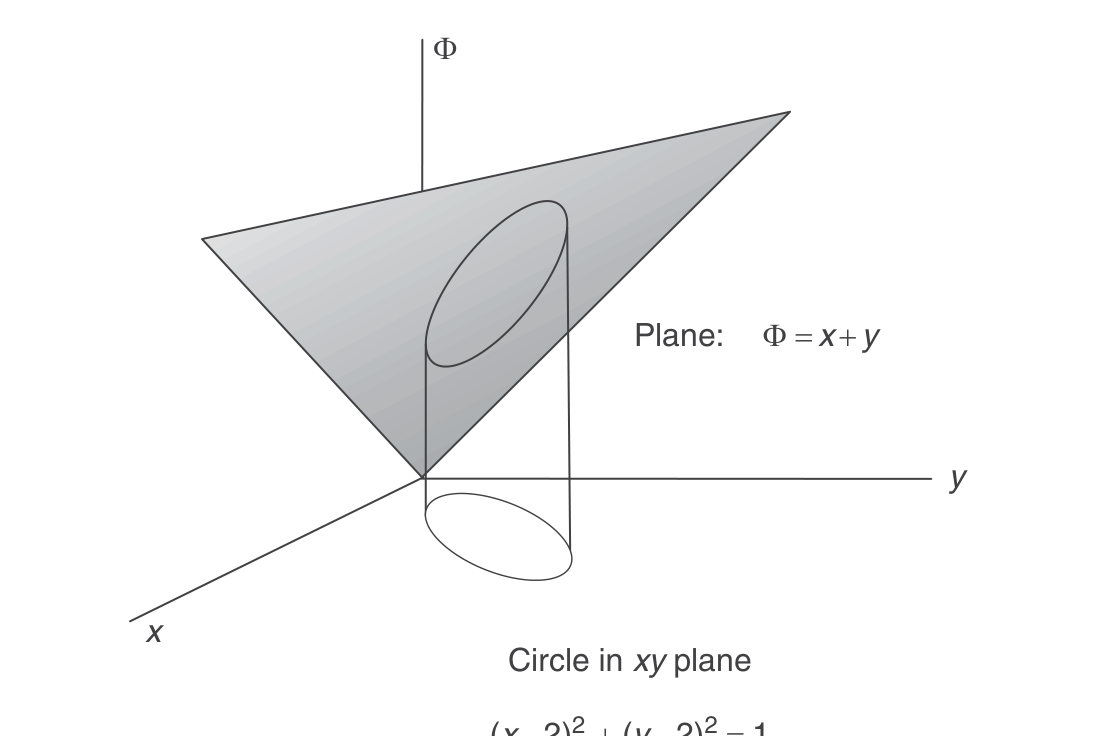
\includegraphics[width=0.55\linewidth]{../Figures/fig_2_5.png}
\caption{Figure 2.5}
\end{figure}

points of the projected circle, given the constraint (x -2)2 + (y -2)2 = 1.
Solution 2.3 Given
(x, y) = x + y,
f (x, y) = (x -2)2 + (y -2)2 -1 = 0,
the condition
\textbackslash{}delta ( + \textbackslash{}lambda f ) = 0,
when inserted into the Euler--Lagrange equation, leads to the following three
equations
\textbackslash{}partial
\textbackslash{}partial x ( + \textbackslash{}lambda f ) = 0 \textbackslash{}implies 1 + \textbackslash{}lambda (2(x -2)) = 0,
\textbackslash{}partial
\textbackslash{}partial y ( + \textbackslash{}lambda f ) = 0 \textbackslash{}implies 1 + \textbackslash{}lambda (2(y -2)) = 0,
\textbackslash{}partial
\textbackslash{}partial \textbackslash{}lambda ( + \textbackslash{}lambda f ) = 0 \textbackslash{}implies (x -2)2 + (y -2)2 -1 = 0.

The third equation is simply the constraint. The first and second equations can
be solved for \textbackslash{}lambda . Equating the two expressions for \textbackslash{}lambda  we obtain
2x -4 =
2y -4
which yields x = y. Inserting this into the third equation we obtain
2(x -2)2 = 1
from which
x = 2 \textbackslash{}pm  1/
\textbackslash{}sqrt
and consequently, the extrema are at
(1.29, 1.29) and (2.71, 2.71).
2.4.2 Non-holonomic constraints
Differential constraints
Suppose the constraint is not an algebraic relation between the variables, but
a differential relation. For example, the ``rolling without slipping'' constraint is
expressed as a relation between the linear displacement and the angular displacement in the form
ds = rd\textbackslash{}theta .
Dividing by dt you note that this is a relationship between velocities rather
than coordinates. Now obviously if you can integrate the relation between differentials, you will get a holonomic constraint, and you can proceed as before.
If the constraint is truly non-holonomic, all is not lost because for some nonholonomic constraints one can apply the Lagrangian \textbackslash{}lambda -method described above.
Assume the constraint is expressed in the form
A1\textbackslash{}delta y1 + A2\textbackslash{}delta y2 + \textbackslash{}cdot  \textbackslash{}cdot  \textbackslash{}cdot  + An\textbackslash{}delta yn = 0.
There are two things to be noted here. First of all, the partial derivatives that
appeared in Equation (2.17) are replaced by the coefficients Ai which are functions of the dependent variables but they are not derivatives of some function.
Secondly, we cannot eliminate a variable because we do not have the equations
between them that we need to eliminate one variable in terms of the others.
Nevertheless, the Lagrangian \textbackslash{}lambda -method can be applied. Define the quantity \textbackslash{}delta f :
\textbackslash{}delta f = A1\textbackslash{}delta y1 + A2\textbackslash{}delta y2 + \textbackslash{}cdot  \textbackslash{}cdot  \textbackslash{}cdot  + An\textbackslash{}delta yn = 0.

2.4
Constraints
Multiply \textbackslash{}delta f by \textbackslash{}lambda  and add it to the variation of the functional :
\textbackslash{}delta  + \textbackslash{}lambda \textbackslash{}delta f = 0.
Now, once again, you can treat all the vis as independent.
If the auxiliary conditions are time dependent (rheonomous) the procedure
is a bit more complicated and we will not consider it. The interested student
may read Section 2.13 of Lanczos3 for a brief discussion.
Isoperimetric constraints
Some constraints are expressed as integrals. Such a constraint is called an
``isoperimetric condition'' because the most famous problem of this type is the
``Queen Dido'' problem of finding the curve of constant perimeter that encloses
the greatest area.4 In general the constraint is given as a definite integral which
has a fixed given value, thus
x2
x1
f (x, y, y′)dx = C,
(2.25)
where C is known. Such a problem is solvable using Lagrange's \textbackslash{}lambda -method.
Assume the integral to be maximized is
I =
x2
x1
(x, y, y′)dx.
(2.26)
For simplicity let us consider a system subjected to a single constraint. (The
generalization to several conditions of the form (2.25) is straightforward.) The
variation of the condition (2.25) is
\textbackslash{}delta
x2
x1
f (x, y, y′)dx =
x2
x1
\textbackslash{}partial f
\textbackslash{}partial y \textbackslash{}delta y + \textbackslash{}partial f
\textbackslash{}partial y′ \textbackslash{}delta y′

dx = 0.
(2.27)
Multiply Equation (2.27) by the undetermined constant \textbackslash{}lambda  and add it to \textbackslash{}delta I to
obtain
\textbackslash{}delta
x2
x1
( + \textbackslash{}lambda f ) dx = 0.
Thus the Lagrangian \textbackslash{}lambda -method implies that the integral
x2
x1
( + \textbackslash{}lambda f ) dx
4 The legend tells us that Queen Dido, escaping from her brother, went to Carthage. She offered
to buy land, but the ruler of the town haughtily told her she could only have as much land as
she could enclose in the hide of an ox. Dido cut the hide of the largest ox she could find into
the thinnest strip possible. The problem is to show that, given the length of the strip, the
largest area is enclosed by a circle.

is stationary and hence the integrand satisfies the Euler--Lagrange equation.
Note that the constraint and the integral of the functional have the same limits
of integration.
\end{example}

\begin{example}
Example 2.4 Determine the shape of the curve of length L that encloses the
greatest area.
Solution 2.4 Recall from the calculus that the area enclosed by a curve C is
given by
Area =  = 1

(xdy -ydx).
Expressing x and y parametrically as x(t) and y(t) we write
= 1


x dy
dt -y dx
dt

dt = 1

(xy′ -yx′)dt.
(Here t is just a parameter -- it is not the time.) The constraint that the curve
has length L is
f =


x′2 + y′2dt -L = 0.
Note that  = (x, y, x′, y′, t) with t as the independent parameter. Since
+ \textbackslash{}lambda f is stationary, it obeys the following Euler--Lagrange equations:
\textbackslash{}partial ( + \textbackslash{}lambda f )
\textbackslash{}partial x
-d
dt

\textbackslash{}partial ( + \textbackslash{}lambda f )
\textbackslash{}partial x′

= 0,
\textbackslash{}partial ( + \textbackslash{}lambda f )
\textbackslash{}partial y
-d
dt

\textbackslash{}partial ( + \textbackslash{}lambda f )
\textbackslash{}partial y′

= 0,
yielding
2y′ -d
dt

-1
2y +
\textbackslash{}lambda x′

x′2 + y′2

= 0,
-1
2x′ -d
dt

2x +
\textbackslash{}lambda y′

x′2 + y′2

= 0.
Integrating, we obtain
2y + 1
2y -
\textbackslash{}lambda x′

x′2 + y′2 = C2,
-1
2x -1
2x -
\textbackslash{}lambda y′

x′2 + y′2 = -C1,

2.5
Problems
where C1 and C2 are constants of integration. Rearranging we write
y -C2 =
\textbackslash{}lambda x′

x′2 + y′2 ,
x -C1 =
\textbackslash{}lambda y′

x′2 + y′2 .
Consequently, squaring and adding yields
(x -C1)2 + (y -C2)2 =
\textbackslash{}lambda 2
x′2 + y′2 (x′2 + y′2) = \textbackslash{}lambda 2,
which is the equation of a circle of radius \textbackslash{}lambda  with center at (C1, C2).
\end{example}

\section*{2.5  Problems}

2.1 Generalize the Lagrange \textbackslash{}lambda -method to a system with n coordinates and m
constraints (m \textless{} n) and show that
\textbackslash{}delta ( + \textbackslash{}lambda 1f1 + \textbackslash{}cdot  \textbackslash{}cdot  \textbackslash{}cdot  + \textbackslash{}lambda mfm) = 0,
where the \textbackslash{}lambda s are obtained from
\textbackslash{}partial
\textbackslash{}partial qi
+ \textbackslash{}lambda 1
\textbackslash{}partial f1
\textbackslash{}partial qi
+ \textbackslash{}cdot  \textbackslash{}cdot  \textbackslash{}cdot  + \textbackslash{}lambda m
\textbackslash{}partial fm
\textbackslash{}partial qi
= 0,
i = n -m + 1, . . . , n).
\section*{2.2  Determine the equation of the curve giving the shortest distance between}

two points on the surface of a cone. Let r2 = x2 + y2 and z = r cot \textbackslash{}alpha .
2.3 Determine the equation for shortest curve between two points on the surface of cylinder (r = 1 + cos \textbackslash{}theta ).
2.4 Consider a solid of revolution of a given height. Determine the shape of
the solid if it has the minimum moment of inertia about its axis.
2.5 Consider the variational problem for variable end points. (a) Let
I =
b
a
(x, y, y′)dx,
where y(b) is arbitrary. Show that
\textbackslash{}delta I = \textbackslash{}eta  \textbackslash{}partial
\textbackslash{}partial y′

b
a
+
b
a
\textbackslash{}partial
\textbackslash{}partial y -d
\textbackslash{}partial
\textbackslash{}partial y′

\textbackslash{}eta dx,
with the condition
\textbackslash{}partial
\textbackslash{}partial y′

x=b
= 0.

r
a
b
A frictionless tunnel for rapid transits between two points on Earth.
(b) Assume y is fixed at x = a but the other end point can lie anywhere
on a curve g(x, y) = 0. Show that in addition to the Euler--Lagrange
condition we have

-y′ \textbackslash{}partial
\textbackslash{}partial y′
\textbackslash{}partial g
\textbackslash{}partial y -\textbackslash{}partial
\textbackslash{}partial y′
\textbackslash{}partial g
\textbackslash{}partial x = 0.
2.6 A frictionless tunnel is dug through the Earth from point a to point b.
An object dropped in the opening will slide through the tunnel under
the action of gravity and emerge at the other end with zero velocity.
The gravitational potential at a point inside the Earth is \textbackslash{}phi  = -Gms/r
where ms is the mass of the material enclosed by a sphere of radius r.
(We are assuming a constant density Earth.) Use polar coordinates and
find the equation of the path that minimizes the time

dt. Determine the
\begin{figure}[h]
\centering
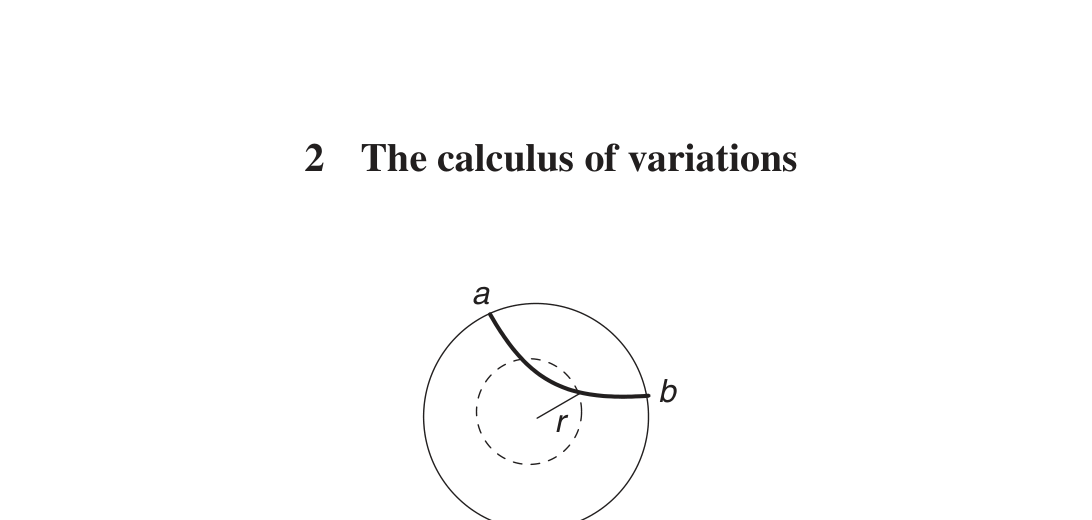
\includegraphics[width=0.55\linewidth]{../Figures/fig_2_6.png}
\caption{Figure 2.6}
\end{figure}

2.7 Two rings of radius a are placed a distance 2b apart. (The centers of the
rings lie along the same line and the planes of the rings are perpendicular
to this line.) Find the shape of a soap film formed between the rings,
noting that the film will have minimal surface area.
\section*{2.8  A particle of mass m is in a two-dimensional force field given by}

F = -GMm
r2 \textbackslash{}hat\{r\}.
The curve requiring the minimum time for the particle to fall from one
point to another is the solution of the differential equation
dr
d\textbackslash{}theta  = f (r).
Determine f (r).
\section*{2.9  Consider the function}

f (x, y, z) = x2 + 2y2 + 3z2 + 2xy + 2xz,
5 See P. W. Cooper, Through the Earth in forty minutes, Am. J. Phys., 34, 68 (1966) and G.
Venezian, Terrestrial brachistochrone, Am. J. Phys., 34, 701 (1966).

2.5
Problems
subject to the condition
x2 + y2 + z2 = 1.
What is the minimum value of f (x, y, z)?
2.10 The speed of light in a medium of index of refraction n is v = c/n =
ds/dt. The time for light to travel from point A to point B is
B
A
ds
v .
Obtain the law of reflection and the law of refraction (Snell's law) by
using Fermat's principle of least time. Using polar coordinates, show that
if n is proportional to 1/r2, that the path followed by a ray of light is
given by sin(\textbackslash{}theta  + c) = kr, where c and k are constants.
2.11 (This is known as ``Newton's problem.'') Consider a solid of revolution
generated by a curve from the origin to a point B in the first quadrant by
rotating the curve about the x axis. It is desired to determine the shape
of this curve if the air resistance on the solid is a minimum. (The solid is
moving towards the left.) Isaac Newton assumed the resistance was given
by the expression
2\textbackslash{}pi \textbackslash{}rho V 2

y sin2 dy,
where  = y′ = the slope of the curve, \textbackslash{}rho  is the air density and V 2 is
the velocity. (This is not a very good expression for air resistance, but
let us assume it is correct.) Obtain an expression for the integral to be
minimized.
\section*{2.12  Determine the curve of length l that joins points x1 and x2 on the axis,}

such that the area enclosed by the curve and the x axis is maximized.
2.13 Determine the shape of a cylinder (that is, the ratio of radius to height)
that will minimize the surface area for a given volume.

This chapter is an introduction to Lagrangian dynamics. We begin by considering d'Alembert's principle and derive Lagrange's equations of motion from
it. We discuss virtual work in detail. Then we present Hamilton's principle and
use it to carry out a second derivation of Lagrange's equations. (This is similar
to the derivation of the Euler--Lagrange equation presented in Chapter 2.) It
should be noted that Hamilton's principle is the fundamental principle of analytical mechanics. The fact that it is deceptively simple should not obscure the
fact that it is very profound. We then consider how to determine the forces of
constraint, and finish up by discussing the invariance of Lagrange's equations.
3.1 The principle of d'Alembert. A derivation of
Lagrange's equations
Recall that the Lagrange equations of motion are
dt
\textbackslash{}partial L
\textbackslash{}partial $\textbackslash{}dot q$i
-\textbackslash{}partial L
\textbackslash{}partial qi
= 0,
i = 1, 2, . . . , n.
(3.1)
In this section we present a simple derivation of Lagrange's equations based
on d'Alembert's principle.
This principle is, in a sense, a re-statement of Newton's second law, but it is
expressed in a way that makes it a very useful concept in advanced mechanics.
For a system of N particles, d'Alembert's principle is
N

\textbackslash{}alpha =1

Fext
\textbackslash{}alpha
-$\textbackslash{}dot p$\textbackslash{}alpha

\textbackslash{}cdot  \textbackslash{}delta r\textbackslash{}alpha  = 0,
(3.2)
where Fext
\textbackslash{}alpha
is the external force acting on particle \textbackslash{}alpha  and $\textbackslash{}dot p$\textbackslash{}alpha  is the change in
momentum of that particle with respect to time. By Newton's second law it
is clear that the term in parenthesis is zero. Therefore, multiplying this term